\section{\scAssesmentHeader{Российской Федерации}}


% \subsection{\scAssesmentBuildingClass}
% % 
% \subsection{\scAssesmentBuildingMetrics}
% 
% ##########-----Регулирование


\subsection{\scAssesmentBuildingLaw}
% 
В части базы обеспечения стандартизацией процессов регулирования энергетической эффективности законодательством России закреплены национальные стандарты,
описывающие нормативные показатели микроклимата \cite{law_RU_RulesCode_BuildingMicroclimateResedentialPublic} с учётом условий от энергетического воздействия внешней среды \cite{law_RU_RulesCode_BuildingClimatology}
и параметры ограждающих конструкций зданий \cite{law_RU_Rules_Code_ThermalPerformance,law_RU_Rules_Code_BuildingEnclosingConstruction}, оптимизация которых позволяет создавать проектные решения построек,
минимизирующие потери тепловой энергии и мероприятия по снижению затрат на обогрев зданий в целом.
В части базы обеспечения методологии законодательство посредством национальных и межгосударственных стандартов определяет принципиальные подходы (на уровне стратегии)
и методики экономической оценки энергетических систем в зданиях.

Основополагающие концепции для принятия решений, связанных c развитием Арктики, исходят из федерального уровня управления и фиксируются в документах стратегического планирования.
Основания разработки нормативно-правовых актов устанавливают Указы Президента РФ или Приказы ведомств.
На период проведения исследования принят Указ Президента РФ от 5 марта 2020 г. N 164 <<Об Основах государственной политики Российской Федерации в Арктике на период до 2035 года>>.
Согласно Указа, устанавливаются такие методы и механизмы регулирования, как:
\begin{itemize}
    \item издание нормативных правовых актов, регулирующих экономическую и иную деятельность в Арктической зоне Российской Федерации;
    \item разработка и реализация стратегии развития Арктической зоны Российской Федерации и обеспечения национальной безопасности на период до 2035 года, стратегии развития арктического туризма в Российской Федерации;
    \item приведение документов стратегического планирования, разработанных в рамках целеполагания, прогнозирования, планирования и программирования на уровне субъекта Российской Федерации, муниципального образования, а также отраслевых документов стратегического планирования в соответствие с настоящими Основами;
    \item создание единой статистической и информационно-аналитической системы в целях осуществления мониторинга социально-экономического развития Арктической зоны Российской Федерации и управления ее социально-экономическим развитием.
\end{itemize}

На федеральном уровне существуют и дополнительно сформированы формализованные структуры, направленные на работу с арктическими территориям:
\begin{itemize}
    \item Министерство иностранных дел Российской Федерации;
    \item Государственная комиссия по вопросам развития Арктики;
    \item Министерство экономического развития России (Департамент развития межрегионального и приграничного сотрудничества);
    \item Комитет по федеративному устройству, региональной политике, местному самоуправлению и делам Севера Совета Федерации Федерального Собрания Российской Федерации;
    \item Совет по Арктике и Антарктике при Совете Федерации Федерального Собрания Российской Федерации;
    \item Комитет по региональной политике и проблемам Севера и Дальнего Востока Государственной Думы ФС РФ;
\end{itemize}
На уровне субъекта Республики Саха (Якутия) авторами установлены следующие формализованные структуры и институции:
\begin{itemize}
    \item Координационный Арктический совет при Главе Республики Саха (Якутия);
    \item Комитет по вопросам коренных малочисленных народов Севера и делам Арктики Государственного Собрания (Ил Тумэн) Республики Саха (Якутия);
    \item Министерство экономики Республики Саха (Якутия) Государственный комитет Республики Саха (Якутия) по делам Арктики.
\end{itemize}
В соответствии с N 190-ФЗ <<Градостроительный кодекс Российской Федерации>> \cite{law_RU_GradoCodex} правовой основой развития территорий являются
документы территориального планирования (Генеральные планы — в случае развития поселений и населённых пунктов),
определяющие стратегию всей административно-территориальной единицы и функциональное назначение территории как класс функциональной зоны,
и документы градостроительного зонирования (Правила землепользования и застройки), устанавливающие правовые возможности и обязанности застройщиков
в форме градостроительных регламентов на предельно допустимые параметры застройки в соответствии с классом территориальной зоны.

В соответствии с № 261-ФЗ <<Об энергосбережении и о повышении энергетической эффективности и о внесении изменений в отдельные законодательные акты Российской Федерации>>
\cite{law_RU_fz_EnergyEff}, ст. 6, допускается передача полномочий органов государственной власти на региональный уровень. При этом органы власти на уровне субъектов и на уровне местного
самоуправления уполномочены разрабатывать собственные программные документы в области энергоэффективного строительства.

Стандарты по развитию ориентированной на человека среды в насёленных местах, в частности --- в городах, --- на период проведения исследования находятся в разработке.
Публичная версия по завершении разработки будет доступна для ознакомления потенциальным инвесторам и интересантам развития территории \cite{law_RU_govAggregatorArcticStandart}.
Разработку «арктического стандарта» ведет АНО «Информационно-аналитический центр
Государственной комиссии по вопросам развития Арктики» под кураторством Минвостокразвития России и Минстроя России.
Техническая реализация представляет комплекс документов, в котором определены основные принципы и подходы к формированию
комфортной городской среды в соотвествии с потребностями и запросами местных жителей, с учётом климатических условий и особенностей социально-экономического развития городов Арктики.
Эти стандарты также нацелены на комплексный подход со включением опыта строительства и объёмно-планировочных решений из традиционных способов возведения северного дома,
которые с течением времени были апробированы и оптимизированы в части энергоэффективности.

Таким образом, акцент регулирования энергоэффективного строительства в Российской Федерации смещён на регулирование посредством механизмов распределения полномочий в соответствии с принципами
местного самоуправления и разработку методических указаний, которые позволят сформировать базу знаний для внедрения в процесс строительства у разнообразных категорий застройщиков.



% ##########-----Опыт


\subsection{\scAssesmentExp}
% 
В Россиской Федерации продолжаются поиский энергетически эффективных подходов в проектировании объёмно-планировочных решений зданий.
Наибольшее влияние на этот процесс оказали разработки В. Щипкова, Б. М. Полуя \cite{1989up_Poluyi_ArchGradoVsurovomKlimate}, К. Г. Туралысова \cite{1996up_Turalysov_BiospherRasseleniye},
труды которых обобщают подходы коренного населения, выработанные при проживании на арктических территориях,
с промышленнными задачами, формирующими требования к расселению, которые были актуальными на период начала промышленного освоения Севера.
В части организации застройки описанные в этих концепциях принципы компактности остаются востребованными и применимыми для формирования энергосберегающей застройки (Рисунок. \ref{fig:st1ch03_ruexp_003}).
\clearpage
\begin{figure}
    \centering
    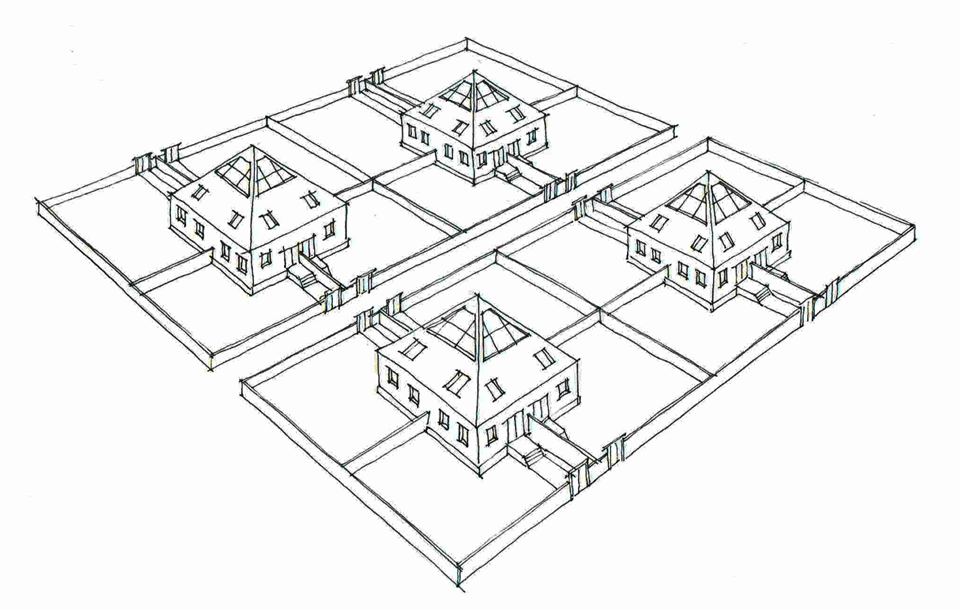
\includegraphics[width=\textwidth]{assets/figures/st1ch03_ruexp_001.png}
    \caption{Концепция компактной энергосберегающей застройки на Севере. Блокированная застройка частными домами}
    \label{fig:st1ch03_ruexp_001}
  \end{figure}

% \clearpage

Принципы энергосберегающей планировки, которые иллюстрируют Рисунки \ref{fig:st1ch03_ruexp_001}, \ref{fig:st1ch03_ruexp_004}, \ref{fig:st1ch03_ruexp_005}, \ref{fig:st1ch03_ruexp_006}, \ref{fig:st1ch03_ruexp_007},
разрабатываемые в рамках концепций застройки, реализуются при вахтовом расслении, на военных базах (Рисунок \ref{fig:st1ch03_ruexp_002}) и научных станциях.


\begin{figure}
    \centering
    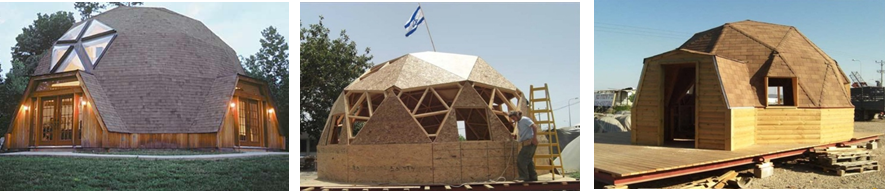
\includegraphics[width=\textwidth]{assets/figures/st1ch03_ruexp_003.png}
    \caption{Уменьшение площади ограждающих конструкций посредством компактной формы постройки в индивидуальном частном домостроении}
    \label{fig:st1ch03_ruexp_003}
  \end{figure}
% \clearpage
\cite{2003buee_Tabunshikov}

\begin{figure}
    \centering
    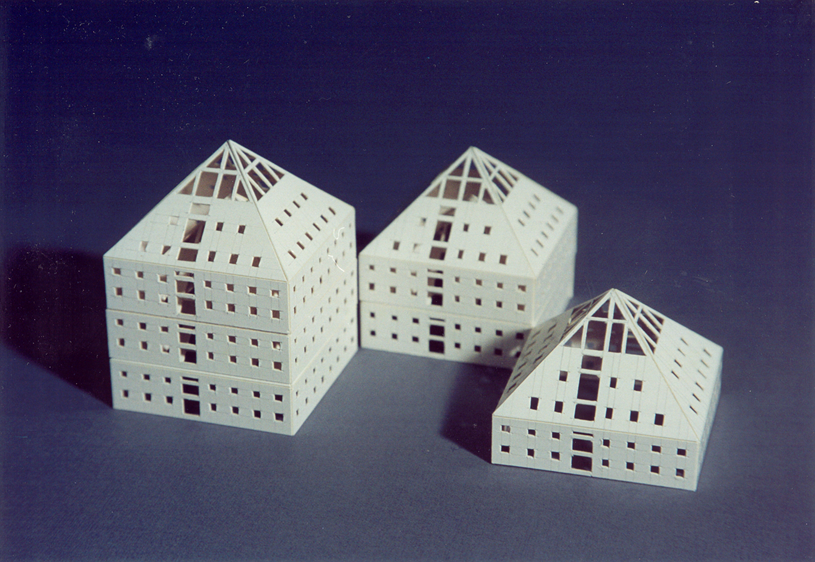
\includegraphics[width=\textwidth]{assets/figures/st1ch03_ruexp_004.png}
    \caption{Концепция компактной энергосберегающей застройки на Севере. Квартирные дома}
    \label{fig:st1ch03_ruexp_004}
  \end{figure}
% \clearpage


\begin{figure}
    \centering
    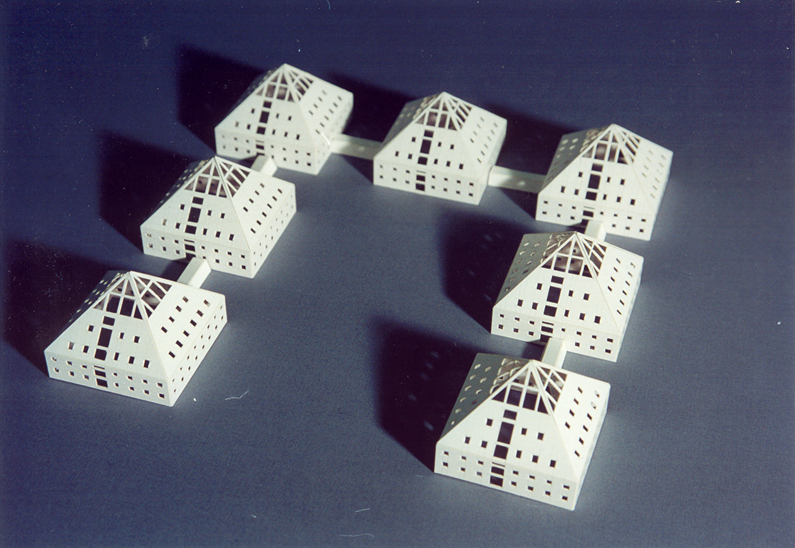
\includegraphics[width=\textwidth]{assets/figures/st1ch03_ruexp_005.png}
    \caption{Концепция компактной энергосберегающей застройки на Севере. Вахтовое расселение}
    \label{fig:st1ch03_ruexp_005}
  \end{figure}


\begin{figure}
    \centering
    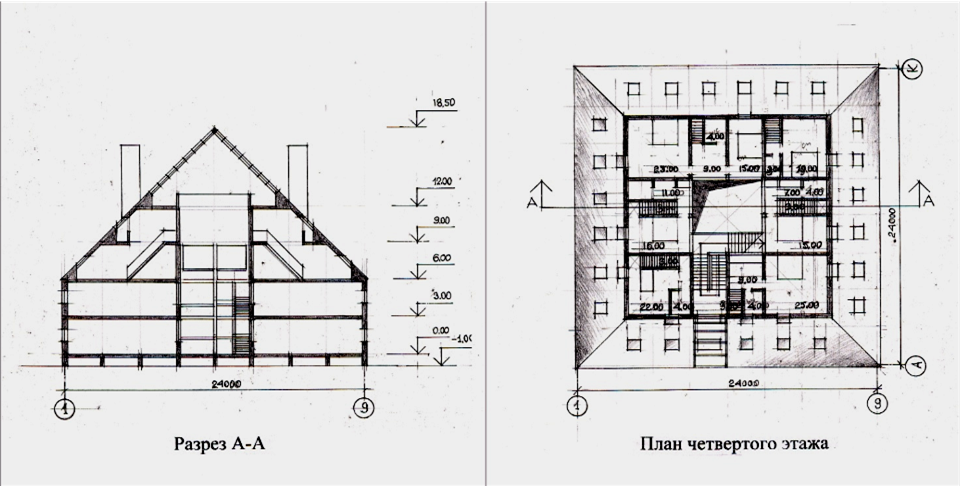
\includegraphics[width=\textwidth]{assets/figures/st1ch03_ruexp_006.png}
    \caption{Концепция компактной энергосберегающей застройки на Севере. Планировочные решения жилого блока}
    \label{fig:st1ch03_ruexp_006}
  \end{figure}


\begin{figure}
    \centering
    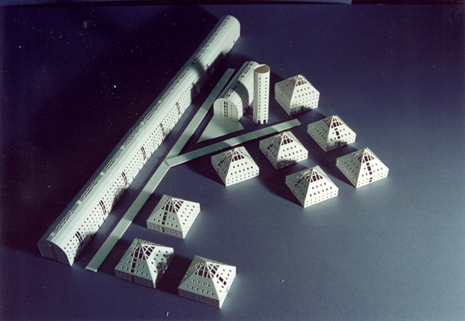
\includegraphics[width=\textwidth]{assets/figures/st1ch03_ruexp_007.png}
    \caption{Концепция компактной энергосберегающей застройки на Севере. Экранирующая противоветровая застройка районов}
    \label{fig:st1ch03_ruexp_007}
  \end{figure}

% \clearpage
\begin{figure}
  \centering
  \includegraphics[width=\textwidth]{assets/figures/st1ch03_ruexp_002.png}
  \caption{Российская военная база <<Арктический трилистник>> на острове Земля Александры (архипелаг Земля Франца Иосифа):
  а - Общий вид военной базы; б, в - Конструктивные особенности военной базы; г - Один из трех эллипсоидных объемов военной базы; д - Интерьер военной базы}
  \label{fig:st1ch03_ruexp_002}
\end{figure}

\begin{figure}
    \centering
    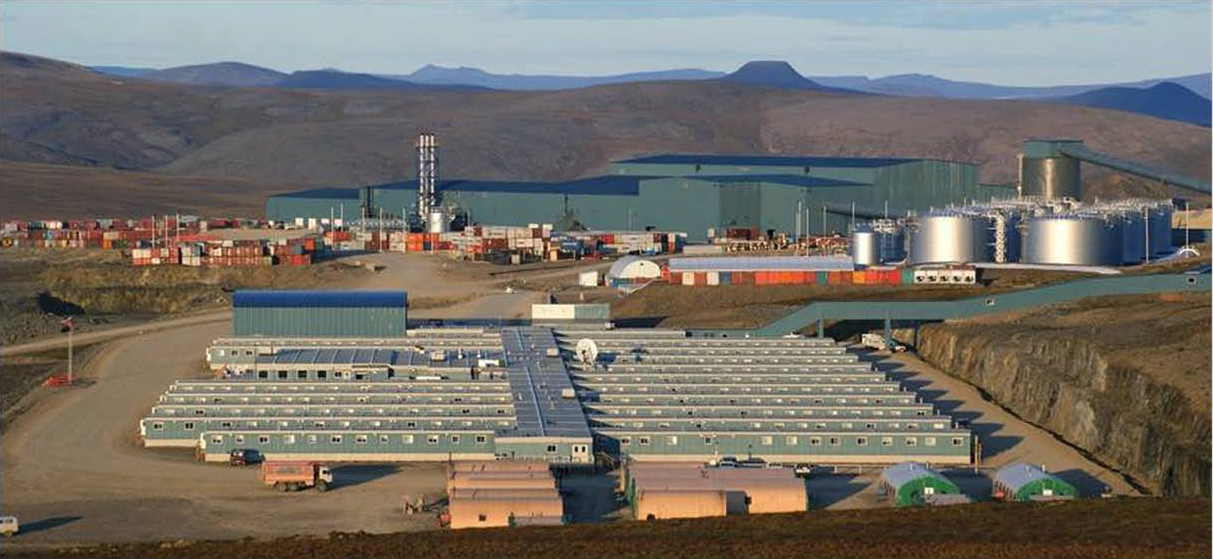
\includegraphics[width=\textwidth]{assets/figures/st1ch03_ruexp_008.png}
    \caption{Вахтовый поселок месторождения Купол, Чукотский автономный округ}
    \label{fig:st1ch03_ruexp_008}
  \end{figure}


\begin{figure}
    \centering
    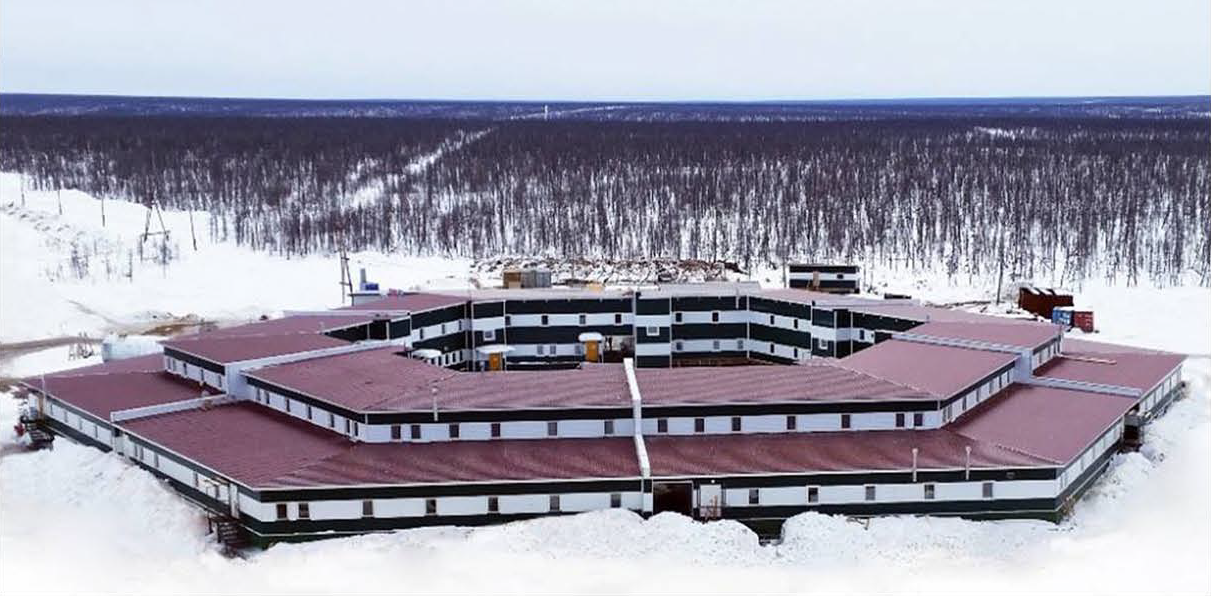
\includegraphics[width=\textwidth]{assets/figures/st1ch03_ruexp_009.png}
    \caption{Вахтовый поселок месторождения Эбелях-Гусиный, Анабарский улус. Республика Саха (Якутия)}
    \label{fig:st1ch03_ruexp_009}
  \end{figure}


\begin{figure}
    \centering
    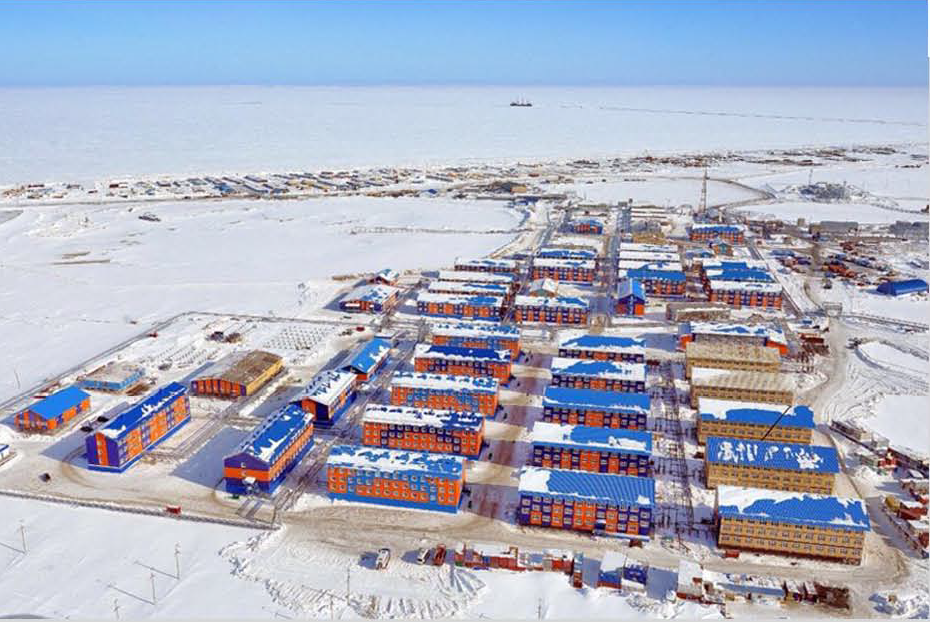
\includegraphics[width=\textwidth]{assets/figures/st1ch03_ruexp_010.png}
    \caption{Вахтовый поселок Сабетта, Ямало-Ненецкий автономный округ}
    \label{fig:st1ch03_ruexp_010}
  \end{figure}

